% ---
\chapter{Fundamentação teórica}
% ---
Neste capítulo será introduzido os conceitos e fundamentos das teorias e tecnologias utilizadas neste projeto. Será abordado sobre autonomia de veículos como o que define um carro autônomo e os diferentes níveis de autonomia. Também abordará o que é um motor de jogo e a principal ferramenta que usaremos para desenvolver um ambiente simulado, a Unity 3D. Por fim, definição de IA, os paradigmas de aprendizado de máquina com um aprofundamento em aprendizado por reforço.

\section{Veículos autônomos}
A SAE (Society of Automotive Engineers) define 6 níveis de autonomia para veículos, do zero ao cinco (\citeonline{SAE2014}). O primeiro, nível zero, não possui automação de direção alguma, é limitado a apenas a tecnologias de assistência como freios ABS ou freio automático emergencial. Um veículo com automação de nível um já passa a possuir alguns recursos que ajudam na direção, como controle para manter o carro na via, controle de velocidade a fim de manter distância de outro veículo a frente. Os níveis dois e três são definidos por, respectivamente, "direção parcialmente automática" e "direção automática condicional", a diferença de ambos pode ser bem sútil, pois em ambos os casos a automação teria o controle do volante, acelerador e freio, no primeiro seria apenas para atividades mais simples, como dirigir na estrada mantendo a velocidade e distâncias, enquanto no nível três o veículo assumiria o controle por um período, podendo até fazer manobras mais avançadas, como ultrapassar um automóvel mais lento a frente. Em ambos os níveis ainda é necessário a atenção máxima do condutor para assumir o controle quando for necessário.

Nos últimos dois níveis de autonomia, temos um veículo que seria capaz de exercer qualquer atividade sem intervenção humana, no nível 4 não seria necessário que o motorista estivesse a condução, só assumiria o controle quando necessário, nesses níveis é capaz inclusive que o automóvel assuma o controle quando necessário, e o mesmo poderia ainda nem possuir volante ou pedais.

Atualmente veículos com autonomia de nível zero a dois, já estão presentes no mercado, nesse artigo estamos interessados em discutir sobre os carros autônomos de nível 3 ou mais, isto é, automóveis que possuam um alto nível de autonomia, o sistema deles podem ser divididos em quatro componentes, cada um deles usam aprendizado de máquina de formas diferentes, são eles: planejamento de rota, decisões comportamentais, controle de moção e controle veicular (\citeonline{Paden2016}). 

O planejamento de rota se trata de definir o trajeto a ser percorrido pelo veículo, isto é, o cálculo do percurso da origem ao destino, imaginar uma cidade com suas ruas, intersecções e pontos de destino como se fosse um grafo ponderado com arestas e vértices e aplicar um algoritmo de busca como Djikstra não é o suficiente para gerar uma solução eficiente, então para isso requer algo que se utilize de outros dados como informação histórica e em tempo real para achar o melhor caminho a ser percorrido em um dado dia da semana, em um dado horário e clima.

Definida a rota, o veículo deve ser capaz de percorrer a mesma tendo em consideração todos os participantes do tráfego e as regras de trânsito, isso envolve uma complexidade de comportamento que vai além de apenas saber conduzir o veículo, então o componente de decisões comportamentais deve saber selecionar ações apropriadas para cada situação. A condução do automóvel em uma rodovia é diferente da condução em um cruzamento em uma rua urbana, onde ele deve parar o veículo e cruzar quando não há nenhum outro veículo ou pedestre no caminho.

A partir do momento que o comportamento foi selecionado, o controle de moção do automóvel autônomo que decide como este vai se locomover, mudança de faixa, conversão a direita, parar o veículo, avançar ao sinal verde, etc, todos essas ações devem ser realizadas de modo que não cause colisões, evitando obstáculos, e devem de ser realizada de forma que não cause desconforto aos passageiros.

O controle do veículo se define pelo controle dos atuadores mecânicos do automóvel para que tenha uma resposta em retorno, essa constante troca de informação é necessária para o controle de moção do veículo atue apropriadamente.

\section{Motores de jogos}
Um motor de jogo (do inglês \textit{game engine}) é um \textit{software} com o objetivo primário de se criar jogos eletrônicos. Estes programas inclui diversas ferramentas que auxiliam o desenvolvedor de jogos a criar seu produto, não existe uma definição sobre quais destas um software deve possuir para ser considerado um motor de jogo, mas frequentemente possuem módulos que lidam com \textit{input} de usuário, renderização de gráficos 2D e 3D, som, motor de física (onde se lida com gravidade e colisão), animação, gerenciamento de memória entre outros (\citeonline{Andrade2015}). 

% Considerar escrever um pouco sobre outros usos de uma game engine aqui, talvez seja necessário para fortalecer o argumento que uma game engine pode ser usada para um simulador e não apenas jogos podendo ter um uso mais "sério"

Como o objetivo é focado no desenvolvimento de uma inteligência artificial para um simulador de carro autônomo, um motor de jogo possui meios que facilitariam o trabalho, não seria necessário desenvolver do zero a renderização dos modelos dos ambientes como veículos, ruas, calçadas, prédios, etc, também não seria necessário desenvolver todo o complexo cálculo de física como força, gravidade, colisão de objetos, peso do veículo, entre outros. Com isso permite que o foco do trabalho a ser feito se limite o máximo possível à análise da IA.

Inicialmente foi considerado o uso de outros motores de jogo, como a Unreal Engine 4 (software da Epic Games, Inc.) e a Godot Engine (Open Source sob licença MIT), embora haja uma preferência natural por uma ferramenta open source do que um software proprietário para realizar esta tarefa, a Unity 3D possui uma comunidade muito maior que o Godot Engine de acordo com (\citeonline{ITCHIO2023}) e (\citeonline{STEAMDB2023}), ambas as fontes são portais que servem para divulgação e venda de jogos publicados por desenvolvedores individuais ou empresas, a Unity 3D é mais utilizada em ambas as plataformas. A Unity 3D possui também seu acervo de recursos criados pela comunidade conhecido como Unity Asset Store onde é possível obter modelos 3D, efeitos sonoros e até modelos genéricos de jogos para se construir algo em cima disso. 

A Unity 3D também possui uma biblioteca de ferramentas própria para criação de agentes inteligentes chamada de \textbf{Unity ML Agent Toolkit}, que foi escrita usando \textbf{Pytorch}, uma biblioteca \textbf{Python} para criação de redes neurais. A Unity ML Agent toolkit oferece um aparato para se criar um agente inteligente, onde é configurado sensores e ações (o que seria a primeira e última camada de uma rede neural) podendo ser treinado usando aprendizado por reforço, por imitação, neuroevolução, entre outros.

\subsection{Editor da Unity3D}
Dentre as principais janelas da interface da Unity3D, temos: hierarquia, projeto, visualização da cena e inspetor. A primeira se trata dos elementos que há dentro da cena (pode-se entender como sendo um trecho do jogo, como este projeto contém apenas uma única cena não é necessário que o leitor entenda tudo que uma cena pode ser), estes elementos são chamados de \textit{GameObjects}, eles são uma abstração de qualquer item dentro do jogo, incluindo o personagem que o jogador controla, o cenário com o qual interage, a "câmera" com o qual o jogo é visto também é um \textit{GameObject}. A primeira janela é chamada de hierarquia porque o conjunto destes objetos podem formar uma estrutura em árvore, por exemplo, podemos criar um objeto "árvore" que conteria os objetos "raiz", "tronco" e "folhas" como seus objetos aninhados. Na seção da proposta é explicado a estrutura deste projeto com mais detalhes.

\begin{figure}[h]
   \centering
   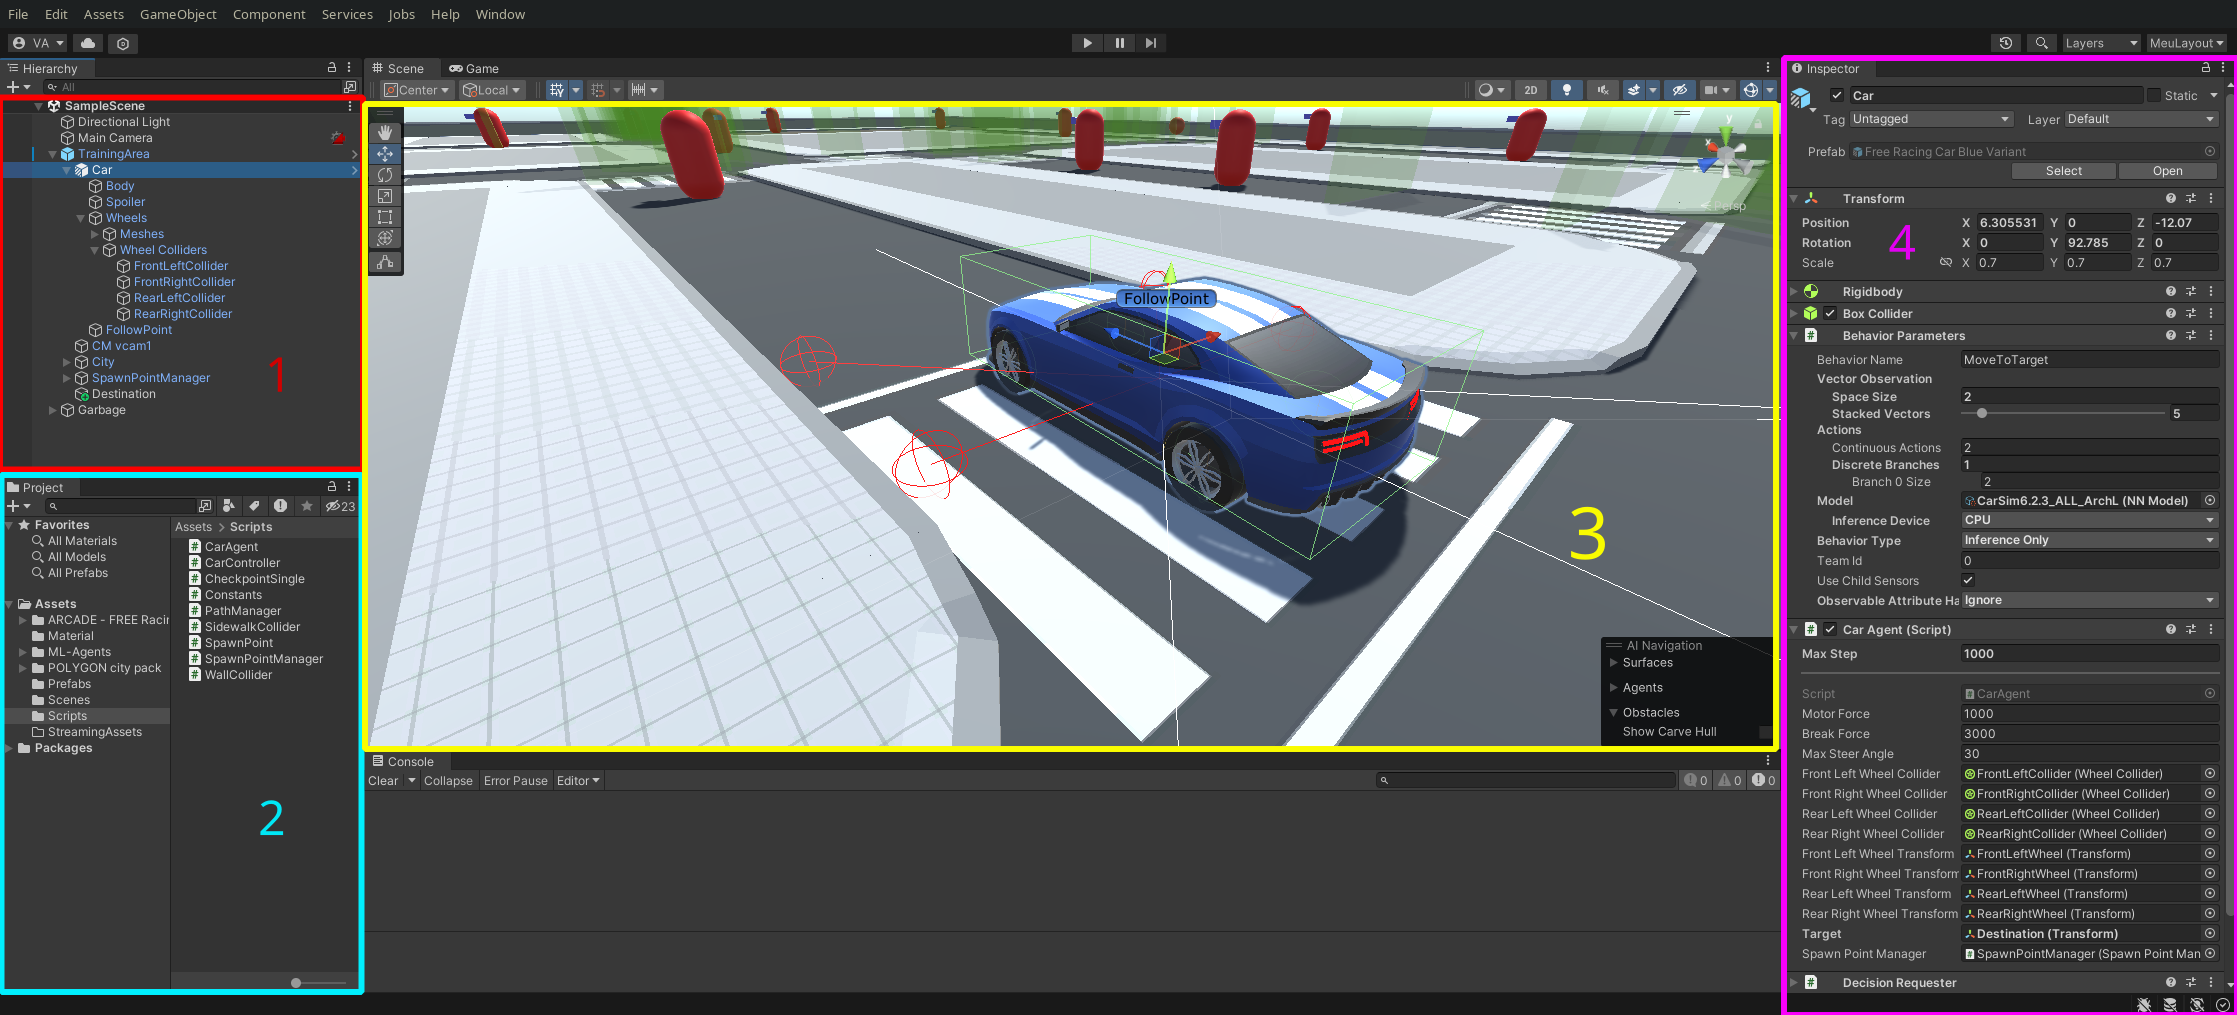
\includegraphics[scale=0.2]{figs/interface-unity3d-indicadores.png}
    \caption{Interface da Unity3D. A janela 1 é a hierarquia, 2 é a janela de projeto, 3 é visualização da cena e 4 é o inspetor}
    \label{fig:unity-ui}
 \end{figure}

A janela de projeto estão os arquivos do projeto, é um diretório do projeto criado pela Unity3D onde deve conter arquivos de efeitos sonoros, códigos-fonte do desenvolvedor, fontes, modelos 2D e 3D, texturas, etc. A visualização da cena é uma janela que permite o desenvolvedor ter uma noção visual da disposição dos \textit{GameObjects}, desta forma ele consegue posicioná-los mais apropriadamente, também consegue ver se a dimensão e escala deles estão coerentes. 

A última janela é o inspetor, nela é exibido os detalhes dos \textit{GameObjects}, isto é, os \textit{components} destes. Como foi explicado anteriormente, os \textit{GameObjects} podem assumir diversas funcionalidades, e são os componentes que permitem isso, por exemplo, o componente \textit{Transform}, comum a todos os objetos da cena define as coordenadas (ou posição) que o objeto se encontrará na cena, sua rotação e escala, já os \textit{components} \textit{Mesh Filter} e \textit{Mesh Renderer} são responsáveis pela renderização 3D de um objeto, isto é, sua forma e aparência.

Os conceitos de como funciona um desenvolvimento de jogo dentro do editor da Unity3D podem não ter ficado claro ao leitor, porém na parte sobre o sistema proposto deste artigo é explicado em mais detalhes a estrutura do projeto.

\section{Inteligência Artificial}
Não existe uma definição única sobre o que é Inteligência Artificial (IA), o mesmo pode ser dito quanto ao seu objetivo. Porém, para compreender melhor o seu escopo, pode-se dizer que está interessada em criar um programa de computador que faça uma ou mais dos seguintes tópicos: pensar humanamente, agir humanamente, pensar racionalmente e agir racionalmente. Pensar pode ser entendido como o processo de pensamento, de compreender e argumentar enquanto agir pode ser entendido como tomar ações e possuir um certo comportamento. Humanamente mediria o quanto a Inteligência Artificial consegue se aproximar de um desempenho humano (agindo ou pensando), e racionalmente é quando há o interesse em pensar ou agir de forma ideal, isto é, que faça "a coisa certa" (\citeonline{Russell2009-dn}).

Uma IA que age racionalmente, pode ser entendido como um programa de computador que toma decisões autonomamente. De fato, qualquer algoritmo pode ser criado para tomar decisões de acordo com uma série de condições, mas é esperado mais de um \textbf{agente racional}, ele é criado para observar o ambiente em que está inserido e tomar decisões por um período prolongado, adaptando-se a qualquer mudança e procurando cumprir seu \textbf{objetivo} fazendo isso de forma ideal, não cometendo erros, e quando estes forem inevitáveis, deverá agir de forma a minimizar o dano causado (\citeonline{Russell2009-dn}).

Para desenvolvimento de um veículo autônomo que este artigo se propõe a estudar, não basta um algoritmo definindo condições e instruções, isto seria uma abordagem insuficiente tanto em eficiência quanto em praticidade em seu desenvolvimento. Seria então necessário uma agente racional, que possua as características descritas no parágrafo anterior, que saiba observar o ambiente em sua volta e \textbf{aprenda} a agir de acordo. A seção abaixo elabora mais sobre esta área específica da Inteligência Artificial.

%-
\subsection{Aprendizado de máquina}
%-
Aprendizado de máquina é qualquer processo automatizado que tem como objetivo reconhecer um padrão dentro de um conjunto de dados (\citeonline{Kelleher2015-iw}), em aprendizado de máquina o projetista cria um agente-aprendiz, fornece os dados e define um objetivo a fim de fazer seu agente melhorar seu desempenho na tarefa após sucessivas iterações observando os dados o tomando decisões. 

Há dois paradigmas em AM que valem a pena ser mencionados brevemente antes de irmos ao que será utilizado no projeto, são eles: Aprendizado supervisionado, não-supervisionado. O primeiro lida mais com problemas de classificação, ao agente é fornecido dados rotulados, e ao analisá-los, se o treino foi efetivo, o agente seria capaz de atribuir um rótulo a um novo registro com uma alta acurácia. O Aprendizado não-supervisionado envolve dados sem rótulos, o objetivo do agente é encontrar uma estrutura oculta que conecte os dados, este processo é chamado de clusterização. Embora possa haver espaço para estes paradigmas no campo de autonomia veicular, eles não estão no escopo deste projeto.

% ---
\section{Aprendizado por reforço}
% ---
No aprendizado por reforço o objetivo é sempre fazer com que o agente aprenda a executar uma tarefa, se trata de ensiná-lo a como fazer. O agente está inserido em um ambiente e a ele é dado um objetivo, com isso ele deve aprender a tomar as decisões corretas nas situações apropriadas visando seu propósito. O aprendiz não é instruído sobre quais ações tomar em dadas circunstâncias, ao invés disso o agente aprenderá a tomar as decisões com base na orientação do treinamento, que envolve em premiá-lo quando agir idealmente ou penalizá-lo caso contrário. Esse parecer que o agente recebe é um valor numérico a ser maximizado por ele, e o dever do projetista é programar os critérios que decidem não somente o que é recompensador ou penalizador, mas o quanto é.

A seguir será formalizado como esse proceso ocorre, toda esta seção é baseada em \citeonline{rl-sutton-barto}, exceto quando abordarmos sobre os algoritmos de otimização de política. É importante esclarecer aqui que a formalização a seguir se trata de tipos de problemas mais simples do que iremos lidar neste projeto, porém essa introdução é necessária para compreender os conceitos mais avançados serão vistos posteriormente.

\subsection{Processo de tomada de decisão} \label{mdp-section}
Neste paradigma, o \textit{agente} toma uma decisão $A_t$ que afeta o \textit{ambiente} o qual está inserido, que retorna a ele um estado $S_{t+1}$ e uma recompensa $R_{t+1}$. O conjunto $S$ representa todos os estados possíveis do ambiente, cada estado $s$ representa toda a observação que o agente tem do sistema. 

\begin{figure}[h]
   \centering
   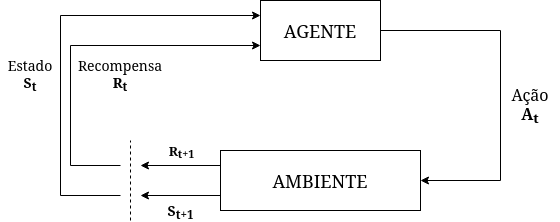
\includegraphics[scale=0.75]{figs/RL-diagram.drawio.png}
    \caption{diagrama da interação do agente com o ambiente. Adaptado de \citeonline{rl-sutton-barto}}
    \label{fig:rl-diagram}
 \end{figure}

Usando o jogo da velha de exemplo, o conjunto $S$ representaria todas as configurações possíveis do tabuleiro, um estado $S_t \in S$ seria um configuração específica, sendo que $S_0$ poderia representar o tabuleiro vazio antes de qualquer jogada. Uma ação $a \in A$ seria uma jogada e por fim $t \in \{0,1,2,3,..., T\}$ as etapas do jogo até a etapa final $T$.

Essa sequência de estados, ações e recompensas é chamada de \textit{trajetória} e pode ser escrita da seguinte forma:

\begin{equation} \label{trajectory}
   S_0, A_0, R_1, S_1, A_1, R_2, S_2, A_2, ... , R_n, S_n
\end{equation}

Esse sistema é conhecido como \textbf{Processo de Decisão de Markov} (\textbf{MDP}, do inglês Markov Decision Process), é uma formalização de problemas que possuem um número \textit{finito} de estados, ações e recompensas, podendo ser \textbf{estocástico}, isto é, não é possível antecipar com exatidão qual será $S_{t+1}$ dado $S_t$ e $A_t$ e de \textbf{tempo discreto}. Dito isso, temos a seguinte distribuição de probabilidade $p$ de um estado $s'$ ocorrer após o agente tomar a decisão $a$ no estado $s$:

\begin{equation} \label{p-definition}
   p(s', r | s, a) \doteq Pr\{S_t = s', R_t = r | S_{t-1} = s, A_{t-1} = a\}
\end{equation}

E por ser uma distribuição de probabilidades, temos: 

\begin{equation} \label{p-sum}
   \sum_{s' \in S}^{} \sum_{r \in R}^{}p(s', r | s, a) = 1 \text{, para todo } s \in S, a \in A(s) 
\end{equation}

Sendo $A(s)$ é o conjunto de todas as ações que podem ser tomadas no estado $s$.

Em um MDP, a probabilidade de cada valor de $S_t$ e $R_t$ depende \textit{apenas} de $S_{t-1}$ e $A_{t-1}$ e de nenhum outro estado anterior a este. Então um estado $S_t$ contém toda a informação de interações passadas entre o agente e o ambiente, essa caraterística do estado é chamada de \textbf{propriedade de Markov}. 

O comportamento do agente é moldado pelas recompensas que recebe a cada ação que toma, este sinal de recompensa é o que indica se o agente está executando a tarefa apropriadamente ou não. Diferente dos estados $S$ e ações $A$, que podem assumir qualquer forma, o conjunto $R$ é um conjunto de números reais: $r \in R \in \mathbb{R}$. A fórmula que deve ser maximizada é chamada de \textbf{retorno esperado}, é denotado por $G_t$:

\begin{equation} \label{expected-return}
   G_t = R_{t+1} + R_{t+2} + R_{t+3} + ... + R_{T},
\end{equation}

onde $T$ é a última etapa que ocorre quando se atinge um \textbf{estado terminal}. Nem todas as tarefas possuem um estado terminal, mas as que têm são chamadas de \textbf{tarefas episódicas}. Usando o exemplo do jogo da velha, podemos entender que cada estado que define um vencedor ou define um empate onde nenhuma jogada mais pode ser feita, seja um estado terminal. Em contraste, se uma tarefa não possui fim, é chamada de \textbf{tarefa contínua}. Como tarefas contínuas teriam $T = \infty$ logo $G_t = \infty$ e se torna impossível calcular por um computador. Então para isso é aplicado um desconto $\gamma$ na equação onde $0 \leqslant \gamma \leqslant 1$:

\begin{equation}
   G_t \doteq R_{t+1} + \gamma R_{t+2} + \gamma^{2} R_{t+3} + ... = \sum_{k = 0}^{\infty}\gamma^{k}R_{t+k+1}
\end{equation}

A \textbf{constante de desconto} $\gamma$ representa o valor de recompensas futuras, caso $\gamma = 0$ o agente apenas se preocuparia em maximizar $R_t$ independente dos valores de recompensas futuras. Quando se aplica um $\gamma$ se aproxima de 1, mais se valoriza estados futuros e aumenta as chances de o agente tomar uma ação que tenha uma recompensa imediata menor mas maiores recompensas futuras. 

Com isso chegamos a uma das partes centrais do RL, que é \textbf{funções valores}. Uma função valor é o que determina o quão importante é para o agente estar naquele estado, isto é, seu valor que é determinado pelo retorno esperado de recompensas futuras daquele estado. Para poder calcular isso é preciso saber como o agente opera, logo, é preciso saber sua \textbf{política}.

A \textbf{política} (representada por $\pi$) é o mapeamento do estado para a ação a ser tomada, formalmente, $\pi(a|s)$ é a probabilidade de se tomar a ação $a$ no estado $s$. Aprendizado por reforço é, basicamente, aprimorar a política do agente e a mesma tende a mudar de uma trajetória para outra (caso episódico) ou até mesmo dentro de uma trajetória.

A definição de uma funcão $v$ valor do estado $s$ sob uma política $\pi$ é:

\begin{equation} \label{state-value-function}
   v_\pi(s) \doteq \mathbb{E}_\pi[G_t|S_t=s]
\end{equation}

Da mesma forma, pode-se estimar o valor de uma ação, para isso há a \textbf{função valor da ação} $q_\pi(s,a)$, definida da seguinte forma:

\begin{equation} \label{action-value-function}
   q_\pi(s,a) \doteq \mathbb{E}_\pi[G_t|S_t=s,A_t=a]
\end{equation}

As funções valores $v_\pi$ e $q_\pi$ podem ser estimadas através de experiência. Pode-se começar com uma política que basicamente atribui a mesma probabilidade para qualquer ação em qualquer estado, conforme as recompensas vão sendo aplicadas o valor esperado do estado e da ação serão atualizados.

\begin{figure}[h]
   \centering
   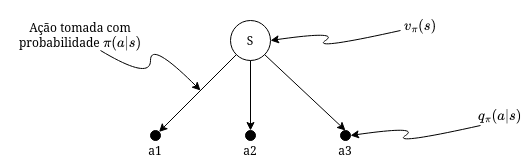
\includegraphics[scale=0.75]{figs/action-selection-diagram.drawio.png}
    \caption{Diagrama das funções valores. Ao estado $s$ é atribuído o valor $v_\pi(s)$, a cada uma das ações é atribuído o valor $q_\pi(a_n|s)$ e tem probabilidade $\pi(a_n|s)$ de ser selecionada. Adaptado de \citeonline{rl-sutton-barto}}
    \label{fig:policy-diagram}
 \end{figure}

Sabemos que $G_t$ é uma função recursiva de modo que $G_t \doteq R_{t+1} + \gamma G_{t+1}$. Com isso é fácil percerber que o mesmo se aplica para as funções valores, para qualquer política $\pi$ em qualquer estado $s$, temos a seguinte função valor recursiva:

\begin{equation}
   \begin{aligned}[b]
      v_\pi(s) &\doteq \mathbb{E}_\pi [G_t | S_t = s] \\
      &= \mathbb{E}_\pi [R_{t+1} + \gamma G_{t+1} | S_t = s] \\
      &= \sum_{a}\pi(a|s) \sum_{s'}\sum_{r}p(s', r | s, a)[r+\gamma\mathbb{E}[G_{t+1}|S_{t+1} = s']] \\
      &= \sum_{a}\pi(a|s)\sum_{s', r}p(s', r | s, a)[r + \gamma v_\pi(s')]\text{, para todo } s \in S
   \end{aligned}
   \label{recursive-state-value-function}
\end{equation}

Resolver uma tarefa por aprendizado por reforço é, grosseiramente, encontrar uma política que retorne uma grande quantidade de recompensa no longo prazo. Um política $\pi$ é dita melhor que outra $\pi'$ se e somente se $v_\pi(s) \geqslant v_{\pi'}(s)$, para todo  $s \in S$. Em um MDP finito, é garantido que haja pelo menos uma \textbf{política ótima}, isto é, uma que seja melhor que qualquer outra para todos os estados, esta política é geralmente representada por $\pi_\ast$, neste caso ela deve utilizar uma \textit{função valor do estado} também ótima:

\begin{equation} \label{state-value-optimal-function}
   v_\ast(s) \doteq \max_{\pi}v_\pi(s) \text{, para todo } s \in S
\end{equation}

similarmente, para acharmos a \textit{função valor da ação} ótima:
\begin{equation}\label{action-value-optimal-function}
   q_\ast(s,a) \doteq \max_{\pi}q_\pi(s,a) \text{, para todo } s \in S \text{ e } a \in A(s)
\end{equation}

% É importante esclarecer aqui que o ato de condução de um veículo \textbf{não é} um problema que pode ser resolvido por MDP, pois possui um número virtualmente infinito de estados e as etapas não são definidas em tempos discretos $t \in \{0,1,2,...\}$. De qualquer forma, é importante discorrer sobre MDPs para se entender o processo de tomada de decisão, o que é política e como otimizá-la.

\subsection{Algoritmos de otimização de política e conceito de aproximação}
% Texto temporário abaixo explicando o que será cobrido nesta seção 
Nesta seção será abordado mais sobre os diferentes tipos de algoritmos de otimização de política, principalmente o PPO, SAC que estão disponíveis no ML-Agents da Unity 3D. 

Existem muitas formas de se chegar aos valores das funções (\ref{state-value-optimal-function}) e (\ref{action-value-optimal-function}) e na política ótima, dentre elas pode-se citar programação dinâmica usando a equação (\ref{recursive-state-value-function}) que é uma \textbf{equação de Bellman}, onde usa-se iteração para avaliar os estados e depois otimizar a política, e com a política otimizada reavalia os estados para então otimizar a política novamente, e assim por diante até que os valores dos estados convirjam para seus "valores verdadeiros". 

%Considerar fazer um resumo melhor sobre Monte Carlo e Q-Learning (exigirá mais leitura, deixar pra dps)
Outro método seria \textbf{Monte Carlo}, que não assume total conhecimento do ambiente (condição necessária para otimizar com programação dinâmica) e utiliza-se de experiência prévia. Por fim temos \textbf{Q-learning} que combina um pouco dos dois. Apesar destes métodos terem suas aplicações, não discorreremos aqui sobre eles, pois, como foi explicado anteriormente, a tarefa que o agente condutor executará não é um MDP finito. 

A condução de um veículo autônomo não possui um número finito de estados, pelo contrário, se considerarmos o uso de visão computacional com processamento de imagem a quantidade de estados possíveis se torna virtualmente infinito. Os problemas que um MDP finito resolve são \textbf{tabulares}, isto é, podem ser dispostos em uma tabela, onde se guardaria a relação com ações válidas, seus valores, etc. Além disso, um estado não irá possuir a \textbf{propriedade Markov}, isto é, não possui informação passadas da interação agente-ambiente.

Para isso há os \textbf{métodos de aproximação}, onde a quantidade de estados possíveis é tão grande que podemos assumir que o agente nunca passará pelo mesmo estado novamente. Portanto, uma abordagem em que alterar um valor $v(s)$ não altera o valor de outro estado semelhante $v(s')$ não parece útil, ao invés disso precisamos assumir que a valorização de um estado implique na valorização de outro. Além disso, temos o fato de que é inviável calcular  $v_\ast(s)$ para todo $s \in S$, então agora será explorado os métodos de \textbf{aproximação}, que se baseia em utilizar uma função valor do tipo $\hat{v}(s, \mathbf{w}) \approx v_\ast(s)$ e $\mathbf{w} \in \mathbb{R}^d$. Dessa forma $\hat{v}$ pode ser tanto uma função linear com $\mathbf{w}$ sendo um vetor dos coeficientes quanto uma rede neural com $\mathbf{w}$ sendo os pesos das conexões.

\subsection{Métodos de gradiente de política e de ator-crítico}
Métodos de gradiente de política são uma abordagem diferente das já mencionadas acima, no caso a atualização da política não depende das funcões valores das ações, em vez disso temos $\pi(a|s, \mathbf{\theta}) = \Pr\{A_t = a | S_t = s, \mathbf{\theta}_t = \mathbf{\theta}\}$ para  a probabilidade de ação $a$ ser selecionada  no tempo $t$ dado que o ambiente se encontra no estado $s$ com parâmetros $\mathbf{\theta} \in \mathbb{R}^{d'}$. Agora o interesse é atualizar $\mathbf{\theta}$ a fim de aprimorar a política da seguinte forma:

\begin{equation}
   \mathbf{\theta}_{t+1} = \mathbf{\theta} + \alpha \widehat{\nabla J (\mathbf{\theta_t})},
\end{equation}

onde $\alpha$ é o tamanho do salto do gradiente e $\widehat{\nabla J (\mathbf{\theta_t})} \in \mathbb{R}^d$ é uma estimativa estocástica cuja expectativa se aproxima do gradiente da medida de desempenho em relação ao seu argumento $\mathbf{\theta}_t$. Qualquer método que obedeça a regra acima é um \textbf{método de gradiente de política} (PGM, do inglês Policy Gradient Method) podendo ou não utilizar de aproximação de função valor do estado $\hat{v}(s)$ descrito acima, caso utilize será considerado um \textbf{método de ator-critico} (actor-critic method). 

Como foi mencionado na introdução, o pacote ML-Agents possui dois algoritmos de aprendizado por reforço: o \textbf{PPO} e o \textbf{SAC}. O primeiro é a sigla para \textbf{Proximal Policy Optimization} e é um PGM que tem o diferencial de que ele alterna entre extrair dados da política e executar uma otimização em lotes dos dados extraídos, além de aproveitar de se aproveitar de TRPO (Trust Regional Policy Optimization) mas sem ser tão complicado quanto. O algoritmo foi criado a fim de ser mais eficiente em processamento de dados e mais robusto (obter sucesso sem ter que ajustar os hiper-parâmetros) (\citeonline{Schulman_Wolski_Dhariwal_Radford_Klimov_2017}).

\textbf{SAC} (ou Soft Actor-Critic) é um algoritmo to tipo off-policy que visa maximizar o retorno esperado e entropia, isto é, obtem progresso agindo mais aleatoriamente possível. Isso é para evitar um problema comum em métodos que lidam com algoritmos de aprendizado de reforço que são livres de modelo: fragilidade a hiper-parametros (quando uma pequena mudança nestes gera um disturbio muito grande no desempenho do treino)(\citeonline{Haarnoja_zhou_Hartikainen_2018})

\section{Aprendizado por Imitação}
Um dos problemas que ocorre com \textbf{AR} é a sua ineficiência no início do aprendizado não haver nenhuma refêrencia e suas ações serem randômicas e por isso existe uma enorme dificuldade em fazer um agente aprender uma tarefa executada por humanos. Para isso existe o Aprendizado por Imitação que se baseia em criar um agente que aprenda através de uma demonstração dada por um especialista (geralemente um humano executando a tarefa), no caso essa demonstração seria uma amostragem de trajetórias feitas por ele.

Há duas abordagens principais para isso: \textbf{Clonagem de comportamento} (\textbf{BC}, do inglês \textit{Behavioural Cloning}) e Aprendizado por Reforço Inverso (\textbf{IRL}, do inglês \textit{Inverse Reinforcement Learning})(\citeonline{1606.03476}).

Behavioural Cloning baseia-se em aprender uma política como se fosse um problema de aprendizado supervisionado tratando a trajetória, um conjunto de pares estado-ação, como uma base de dados rotulada (\citeonline{Pomerleau1991}).

Inverse Reinforcement Learning busca a função de recompensa usando a experiência do especialista.
